\chapter{實驗與效能評估}
\label{chapter:evaluation}

% https://hackmd.io/@calee/HkNQc2ByO/https%3A%2F%2Fhackmd.io%2FyR2SvjqNQayQeWL2onkvmg
% https://docs.google.com/spreadsheets/d/11vgvawzM0E8TF6rnjfOtI_Z4iHDMS9jvwvSfVkNA-jU

為驗證本論文設計之方法,將 free5GC 核心網路移植至 OpenNetVM,使用其所提供之 ABI 能有效提升核心網路之效能,本實驗分別對原生之 free5GC 核心網路部屬於 Ubuntu Linux,與經過 OpenNetVM 移植過後之 free5GC 核心網路一樣部屬於 Ubuntu Linux,分別對其控制端 (control plane) 與用戶端 (user plane) 之效能進行測試,最終比對其結果,以驗證經過 OpenNetVM 移植過後的 free5GC 核心網路確實能有效提供更好的性能。

\textbf{Baseline:} 實驗過程我們會分別對原生之 free5GC 與經過移植至 OpenNetVM 的 \LHCN 進行註冊流程、連線建立流程、與換手流程等三個流程作測試,並比較其控制層的效能分析,另外我們也會建立連線後的用戶端進行頻寬測試,最後我們也會比較基於 Berkeley Socket 與基於 OpenNetVM shared memory 的 SBI 的效能差別。

\section{實驗環境設定}
\label{sec:evaluation_env}

我們所使用的硬體與軟體規格如下表~\ref{tab:sys_env}。 \cnote{調 tab:sys\_env 位置}

% This LaTeX table template is generated by emacs 27.2
\begin{table}[htbp]
    \centering
    \begin{tabular}{|c|c|l|}
        \hline
        \textbf{節點} & \textbf{項目} & \multicolumn{1}{c|}{\textbf{規格、型號、說明}} \\
        \hline
        \multirow{6}{*}{\shortstack[c]{Node 1\\ \\Traffic}} & CPU & Intel(R) Core(TM) i7-7700 CPU @ 3.60GHz \\
        \cline{2-3}
        & Core No. & 4 \\
        \cline{2-3}
        & NIC & Intel Corporation Ethernet Controller X710/X557-AT 10GBASE-T \\
        \cline{2-3}
        & OS & Ubuntu 18.04.5 LTS \\
        \cline{2-3}
        & Kernel & 5.4.0-60-generic \\
        \cline{2-3}
        & Software & MoonGen Packet Generator~\cite{github.MoonGen} \\
        \hline
        \multirow{8}{*}{\shortstack[c]{Node 2\\ \\CN}} & CPU & Intel(R) Core(TM) i7-9700 CPU @ 3.00GHz \\
        \cline{2-3}
        & Core No. & 8 \\
        \cline{2-3}
        & NIC & Intel Corporation Ethernet Controller X710/X557-AT 10GBASE-T \\
        \cline{2-3}
        & OS & Ubuntu 20.04.1 LTS \\
        \cline{2-3}
        & Kernel & 5.4.0-65-generic \\
        \cline{2-3}
        & \multirow{3}{*}{Software} & free5GC v3.0.4 \\
        & & HL5GC \\
        & & RAN UE Simulator \\
        \hline
        \multirow{5}{*}{\shortstack[c]{Node 3\\ \\DN}} & CPU & Intel(R) Core(TM) i5-4460  CPU @ 3.20GHz \\
        \cline{2-3}
        & Core No. & 4 \\
        \cline{2-3}
        & NIC & Intel Corporation Ethernet Controller 10G X550T \\
        \cline{2-3}
        & OS & Ubuntu 18.04.5 LTS \\
        \cline{2-3}
        & Kernel & 5.4.0-62-generic \\
        \hline
    \end{tabular}
    % [] 放的是顯示在 list of figure 的文字
    % {} 放的是顯示在圖下方的文字
    \caption[系統環境參數]{{\footnotesize 系統環境參數}}
    \label{tab:sys_env}
\end{table}

我們的實驗在邏輯上 (logically) 將系統分為三個部件,邊緣端 (edge)、核心網路 (core network)、與數據網路 (data network)。邊緣端在真實網路下即是手機、基地臺與相關部件,以下會以 UE-RAN simulator 代稱。核心網路如第二章節所講解的,是第五代行動通訊網路中,放在機房 (data center) 中,負責統籌處理控制端 (control plane) 與轉發 (forward)、封裝 (encapsulate)、解封裝 (decapsulate) 使用者端 (user plane)。而數據網路 (data network),則是泛指傳統網路 (Internet),即為大多數時候,手機使用者想要存取的服務之所在位置。

為了準確的區分流量產稱與流量轉送的中央處理器 (以下簡稱 CPU) 使用率,避免單一 CPU 需要同時產生流量與處理流量,我們的測試方法將流量產生器 (traffic generator)、核心網路、流量接收者 (traffic receiver) 分別部屬於不同的機器上,讓三者得以完全妥善使用三顆不同之 CPU。

因此在務實面 (physically) 上將系統切分成三個節點,分別模擬使用者端流量發送、基地臺與核網處理、資料網路回覆 (圖~\ref{fig:eva_node}),在節點與節點中我們都是使用 Intel 的 10Gbps 雙孔網卡與 CAT-6A RJ45 網路線連接。在 Node 1 上面我們使用 MoonGen~\cite{paper.MoonGen} 軟體來產生流量。在 Node 2 上面我們分別佈署原生的 free5GC v3.0.4 與修改過後的 \LHCN 作為核心網路測試,另外比較特別的是,我們也把自行開發的 RAN UE 模擬器佈署在 Node 2 上面而非 Node 1 上,此模擬器會模擬 5G SA 的控制訊號與核心網路建立連線。而在 Node 3 上主要模擬資料網路回復封包,但若是測試單純下行流量,則會在 Node 3 上啟動 MoonGen 來產生流量。

\cnote{改圖}
\begin{figure}[htbp]
    \centering
    \begin{tikzpicture}
        \tikzset{vertex/.style = {shape=rectangle,draw,minimum size=1.5em,align=center}}
        \tikzset{edge/.style = {<->,> = latex'}}
        % vertices
        \node[vertex] (a) at (10,) {Node 1\\Traffic Generator};
        \node[vertex] (b) at (15,) {Node 2\\Core Network};
        \node[vertex] (c) at (20,) {Node 3\\Data Network};
        %edges
        \draw[edge] (a) to (b);
        \draw[edge] (b) to (c);
    \end{tikzpicture}
    % [] 放的是顯示在 list of figure 的文字
    % {} 放的是顯示在圖下方的文字
    \caption[實驗環境節點]{{\footnotesize 實驗環境節點}}
    \label{fig:eva_node}
\end{figure}

\section{用戶層效能分析}
\label{sec:up_evaluation}

\subsection{上行流量分析}
\label{subsec:uplink_evaluation}

在用戶端的測試中,我們首先作了上行流量測試,分別使用不同大小的 ping 封包從 Node 1 藉由 Node 2 送至 Node 3,在這個測試中關閉 Node 3 回復 ping 的功能,觀察 Node 3 接收到的流量。

\begin{figure}[htb]
    \centering
    % 圖片的高度與寬度, height 設為 ! 代表由寬度大小等比例縮放
    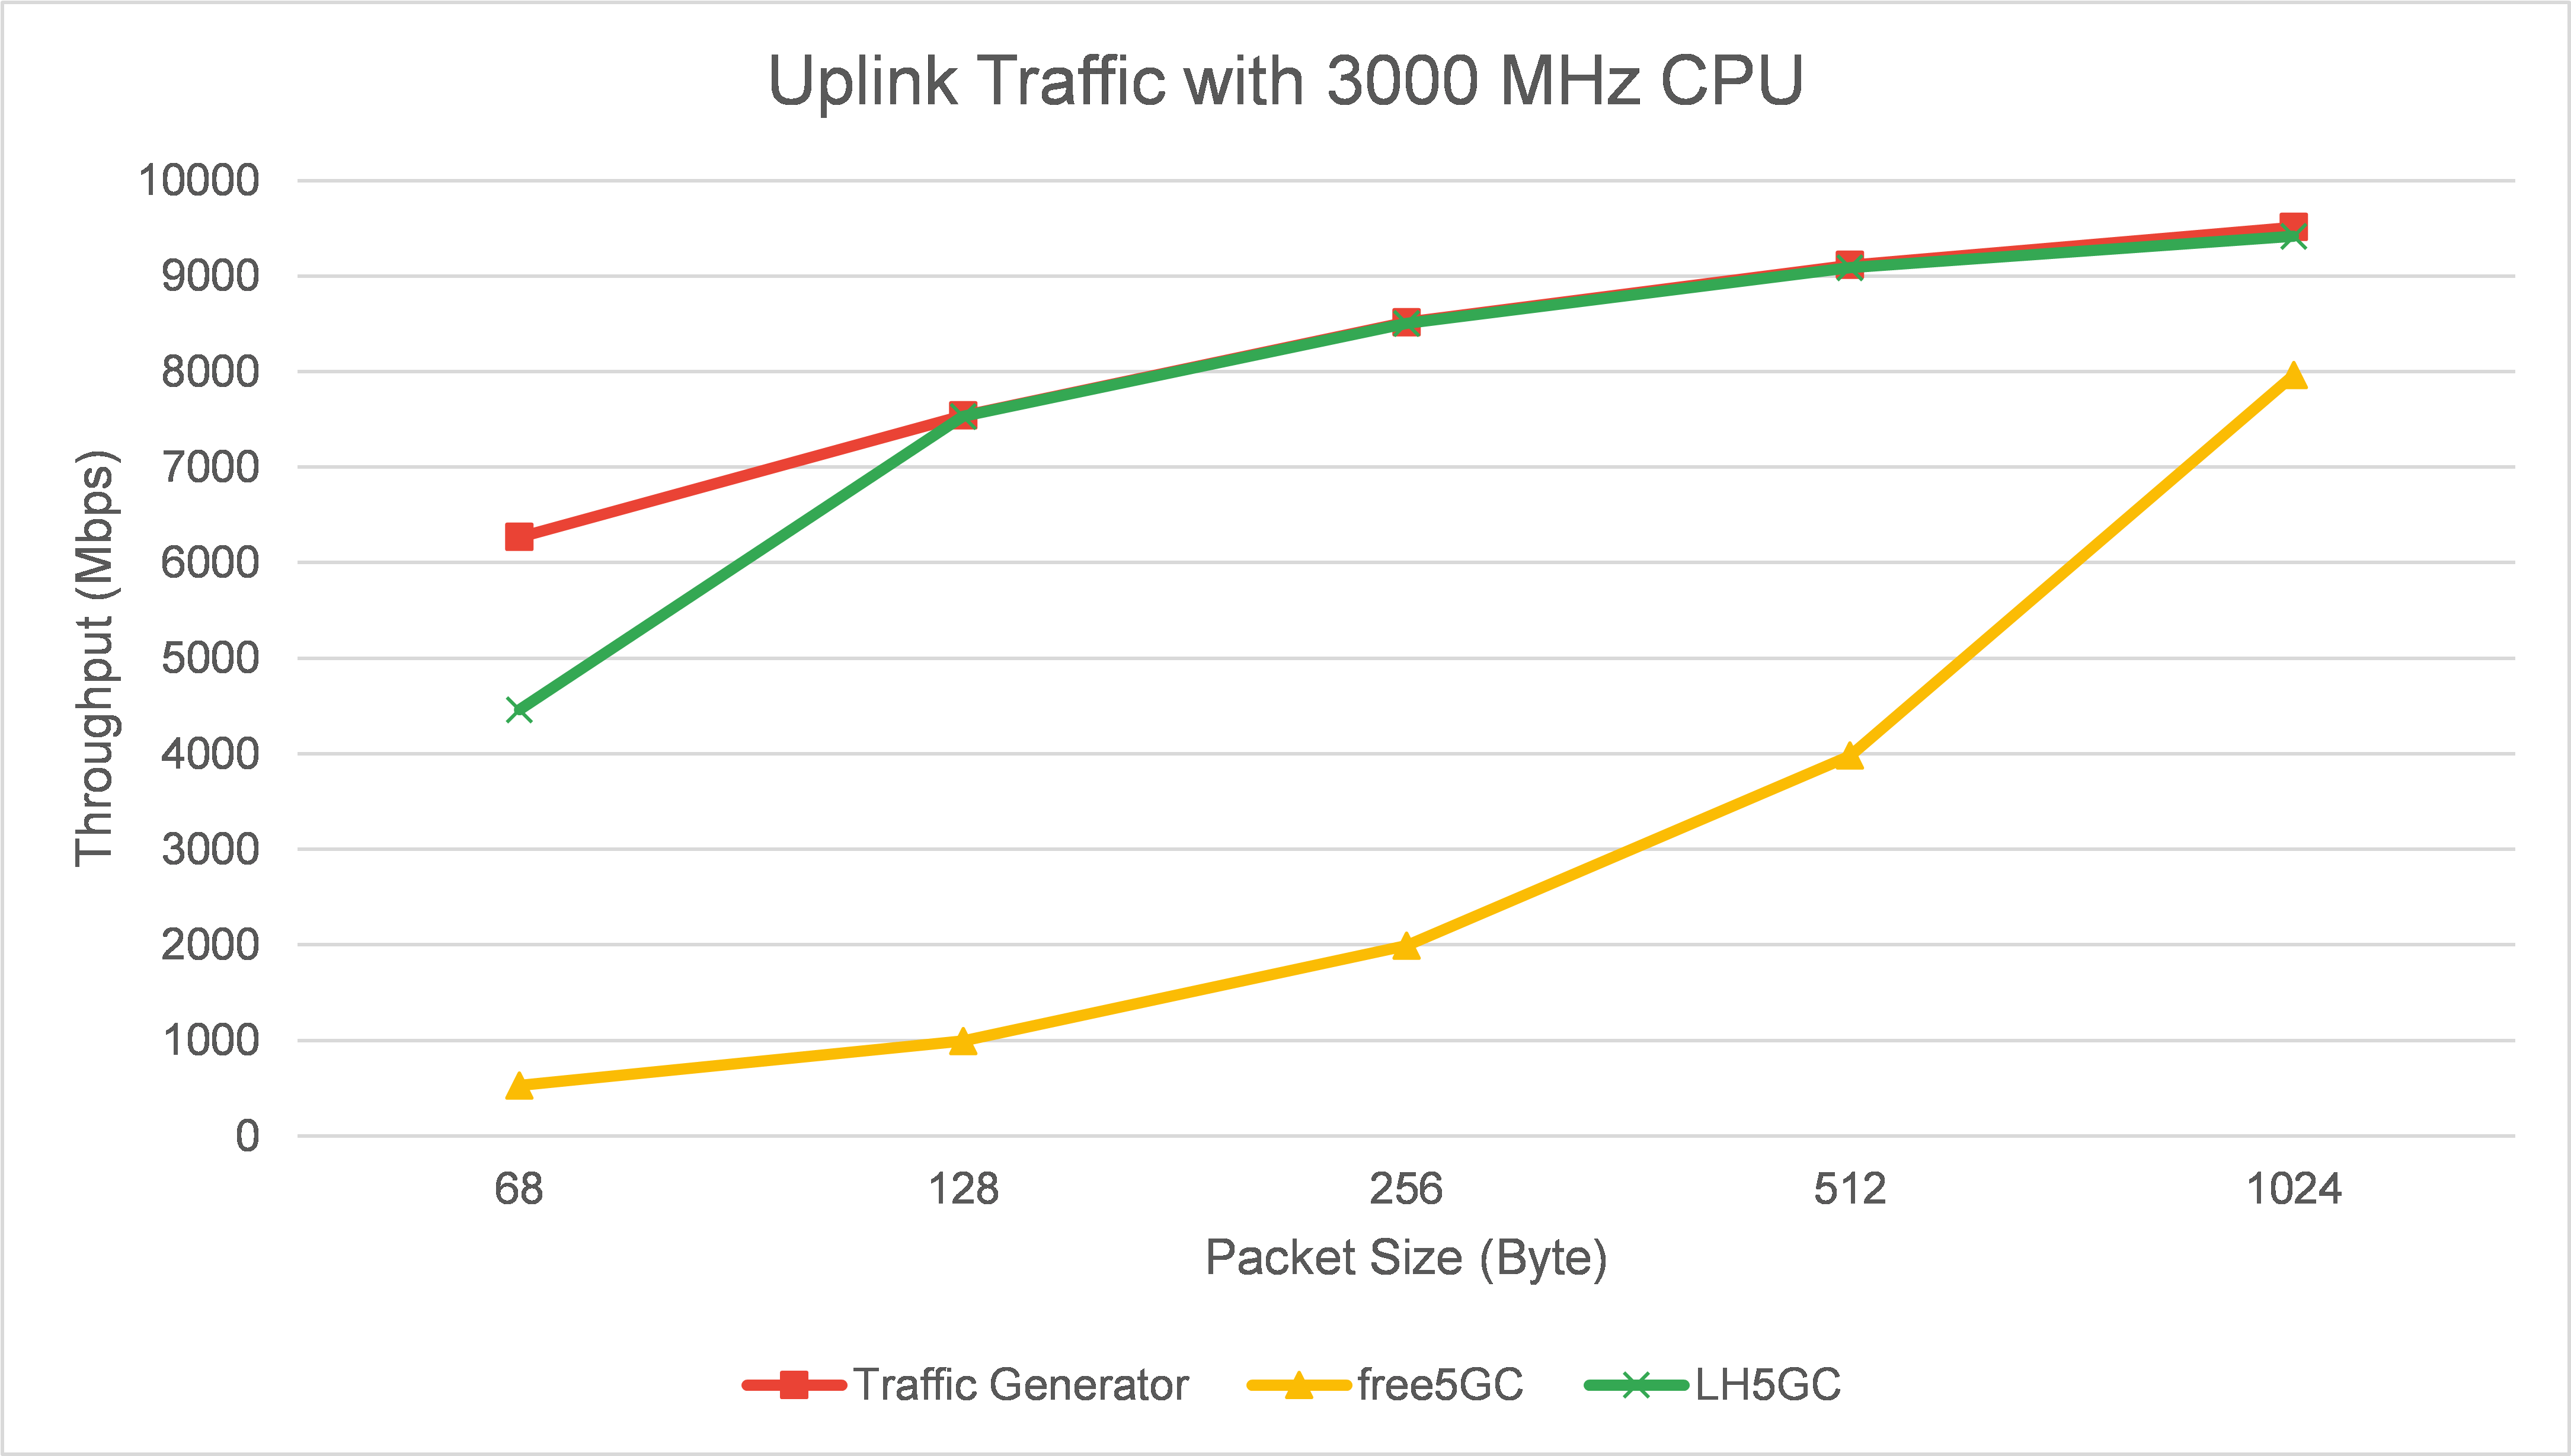
\includegraphics[height=!,width=0.8\linewidth,keepaspectratio=true]{figures/up_eva_pkt_size}
    % [] 放的是顯示在 list of figure 的文字
    % {} 放的是顯示在圖下方的文字
    \caption[用戶層上行效能比較]{{\footnotesize 用戶層上行效能比較}}
    \label{fig:up_eva_pkt_size}
\end{figure}

圖~\ref{fig:up_eva_pkt_size}的縱軸是吞吐量,單位為每秒處理的總位元組,固定 CPU 時脈於 3000 MHz 並比較不同封包大小的影響。由途中可以很明顯的看出 \LHCN 用戶端流量處理能力遠高於 free5GC。在封包大小為 68 位元組 (Byte) 時,\LHCN 的吞吐量會是 free5GC 的十一倍之多,另外在封包大小大於 128 位元組後,\LHCN 的吞吐量會幾乎逼近原始產生的流量,足見得其效能並沒有達到 \LHCN 的流量上限,而是受制於網卡的處理能力。另外隨著封包大小的提升,free5GC 的吞吐量會有明顯的提升,其歸因於核心實作的單位時間封包處理數以達到其固定量。

\subsection{來回流量比較}
\label{subsec:uldl_comp}

在這個測試中,我們比較 \LHCN 與 free5GC 上下行流量,除了關閉 Node 3 ping 回復功能的測項外,也測試了開啟回復功能後,Node 1 接收到的流量。

\begin{figure}[htb]
    \centering
    % 圖片的高度與寬度, height 設為 ! 代表由寬度大小等比例縮放
    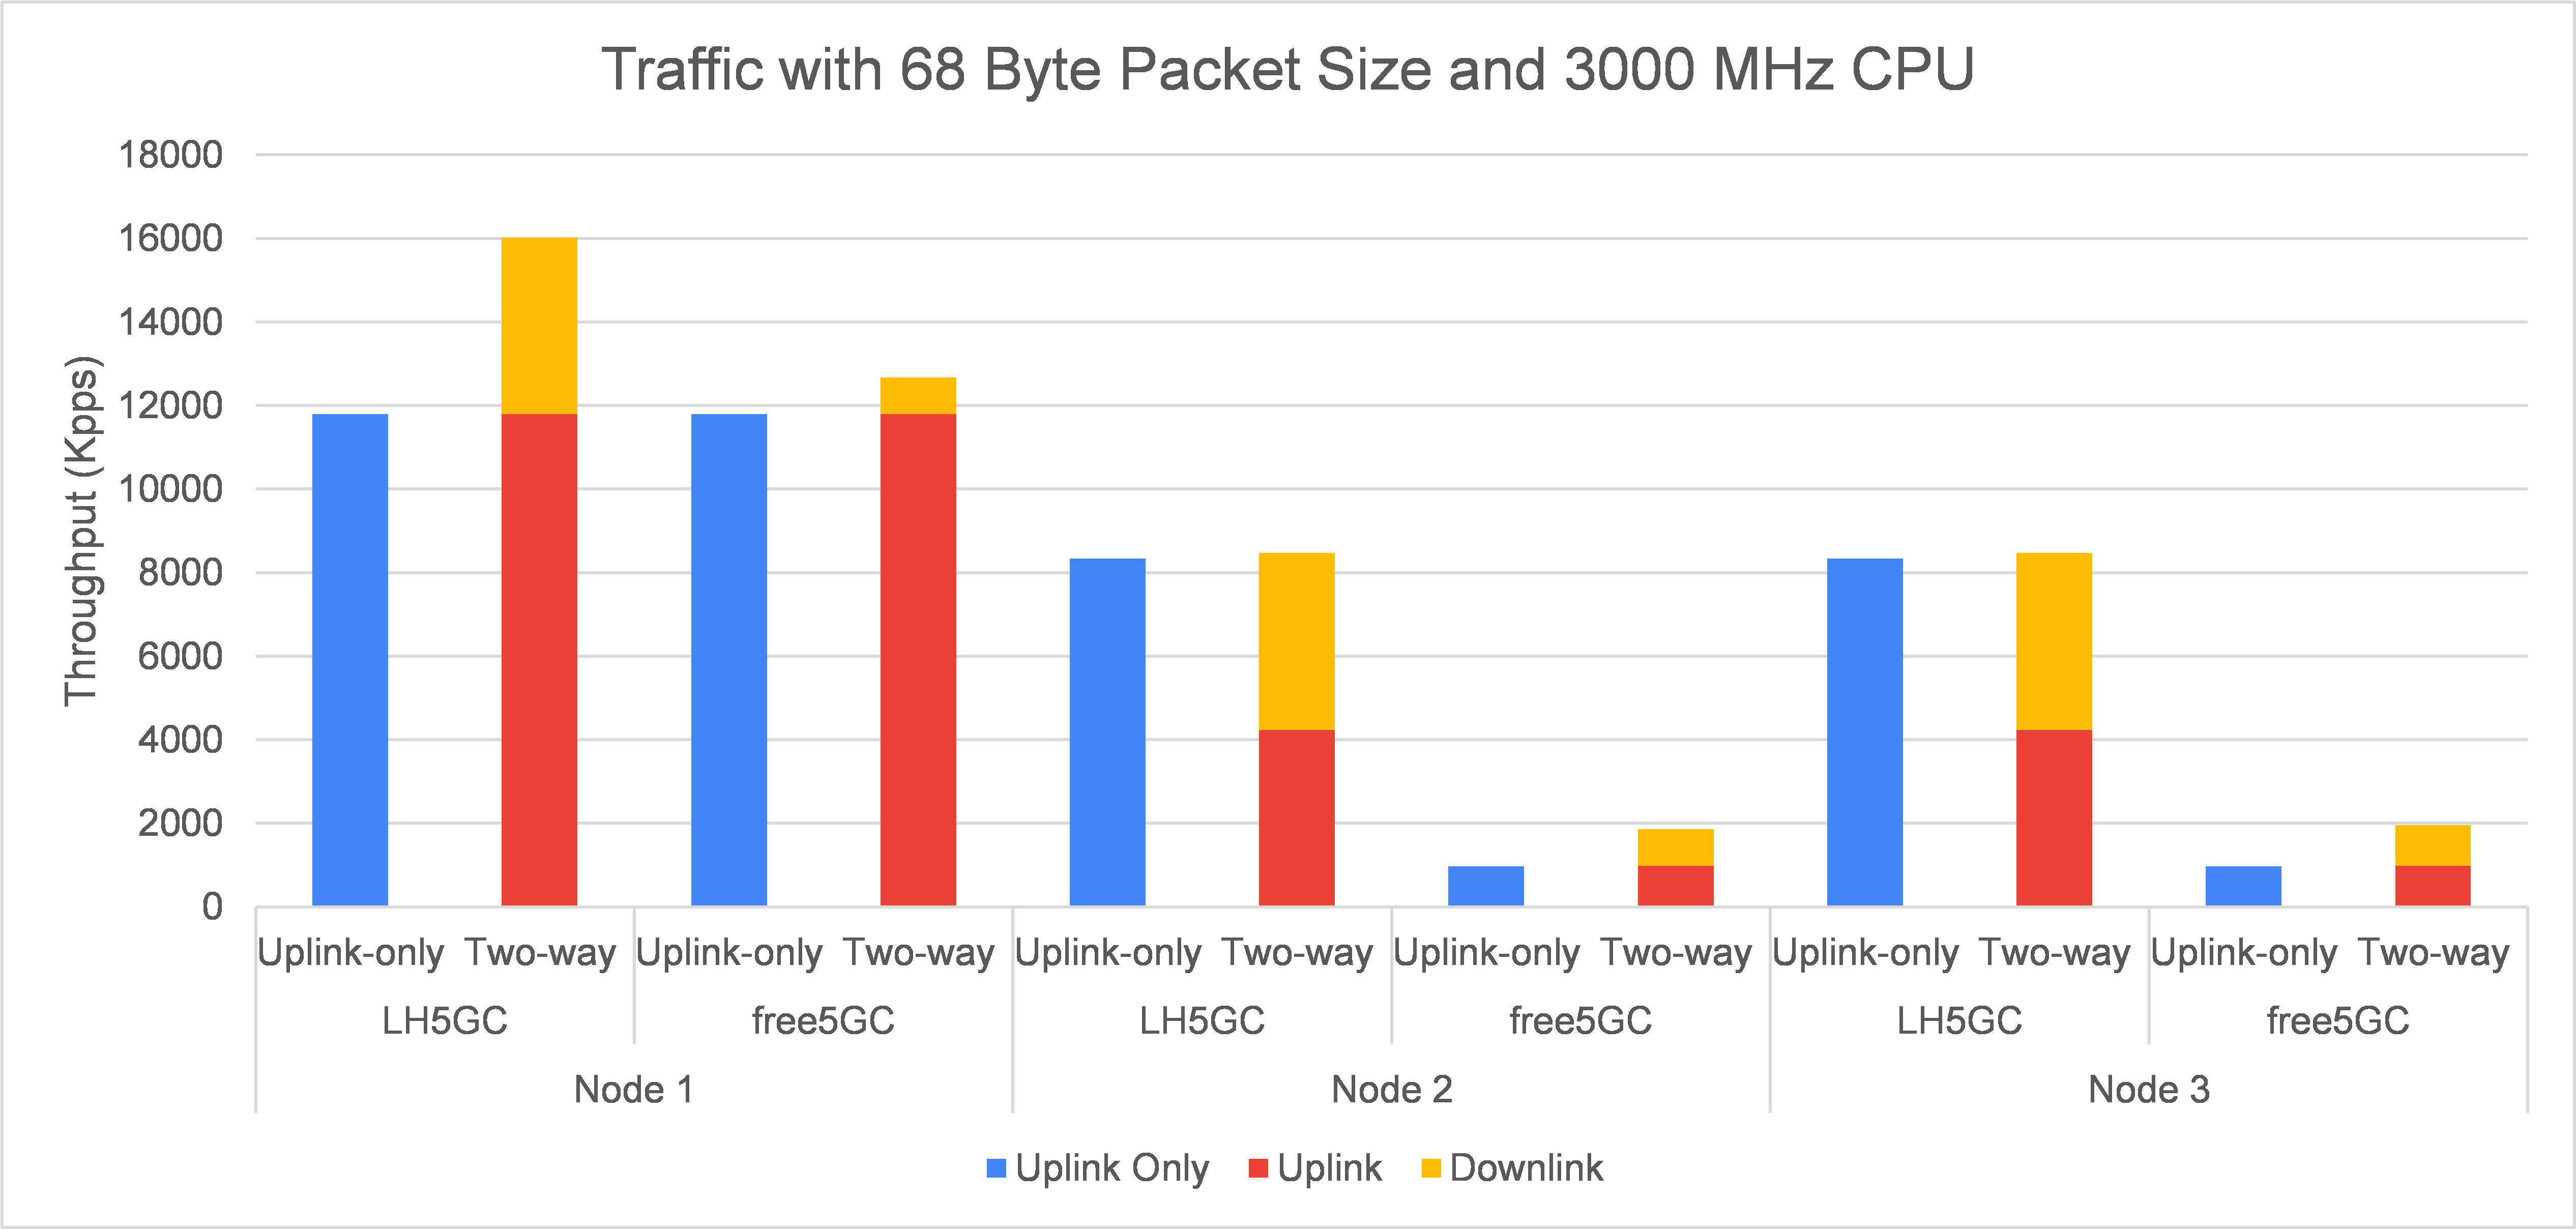
\includegraphics[height=!,width=1\linewidth,keepaspectratio=true]{figures/up_uldl_comp}
    % [] 放的是顯示在 list of figure 的文字
    % {} 放的是顯示在圖下方的文字
    \caption[用戶層上下行比較]{{\footnotesize 用戶層上下行比較}}
    \label{fig:up_uldl_comp}
\end{figure}

圖~\ref{fig:up_uldl_comp}在固定 CPU 時脈於 3000 MHz 並使用 68 位元組的封包,比較 \LHCN 與 free5GC 分別在 Node 1、Node 2、與 Node 3 的上下行流量,藍色長條顯示當只有測試上行時的流量,而紅、黃色長條則是在同時有上下行流量時,其各自的流量大小,縱軸為吞吐量,這裡單位取每秒處理的封包數量。可以看到當流量從 Node 1 被產生到送到 Node 2 處理時,free5GC 所能承受的封包數量足足八倍有餘,而當封包回復至 Node 1 時,\LHCN 的流量會是原本送出時的 $\dfrac{1}{3}$,而 free5GC 則會是降低成原來的 $\dfrac{1}{13}$ (比較 Node 1 紅、黃值條的差距)。

另一個有趣的觀察是於 Node 2 比較單獨上行與上下行流量分配的差異,\LHCN 在單獨上行可處理的封包量約等於同時處理上下行的封包量,而 free5GC 則是可以處理加倍的吞吐量。推測是由於受益於 Kernel Socket 的實作在同時處理上下行時可以分別使用不同的 Kernel Thread 處理,而 \LHCN 由於是透過 DPDK 實作,會搶佔單獨一個 CPU 核心進行網卡封包的輪詢,因此若需要同時處理上下行,亦會受限於單一核心的輪詢能力。

\subsection{CPU 時脈影響}
\label{subsec:cpu_clock}

由於在測試的過程中,我們發現 CPU 時脈會對劉量產稱可觀的影響,因此我們也嘗試測試 CPU 時脈與流量的關係。

\begin{figure}[htb]
    \centering
    % 圖片的高度與寬度, height 設為 ! 代表由寬度大小等比例縮放
    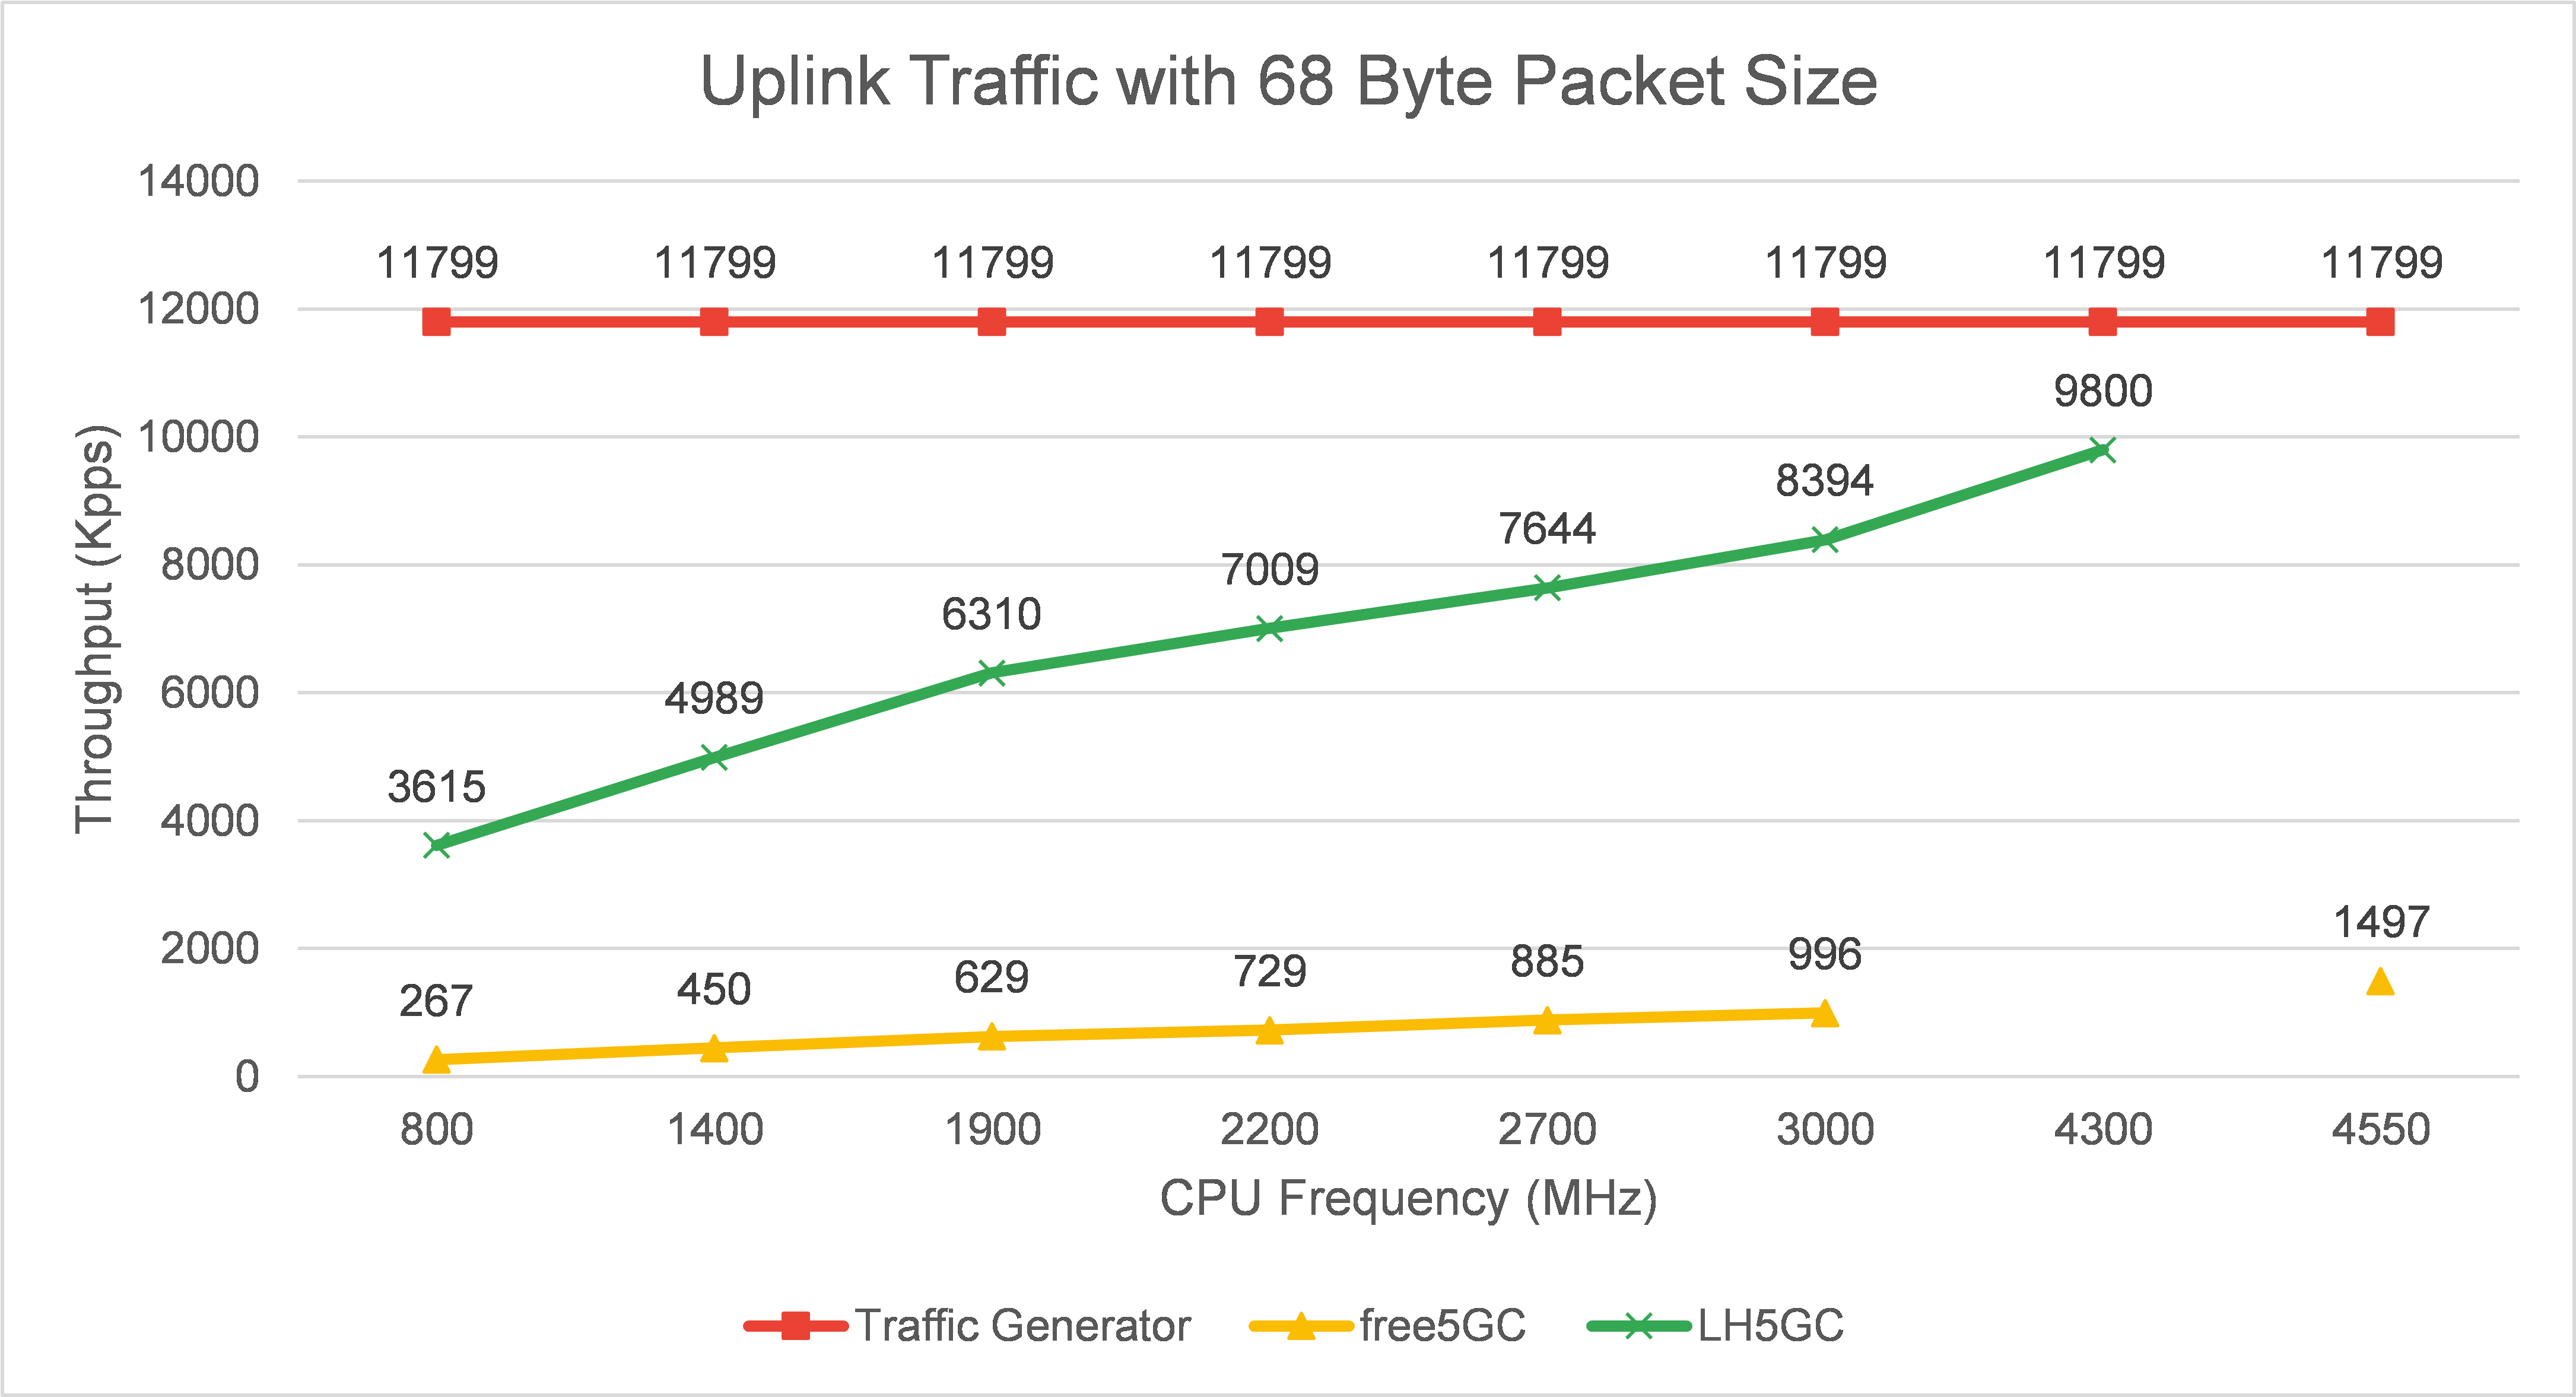
\includegraphics[height=!,width=0.8\linewidth,keepaspectratio=true]{figures/up_cpu_clock}
    % [] 放的是顯示在 list of figure 的文字
    % {} 放的是顯示在圖下方的文字
    \caption[用戶層受時脈影響分析]{{\footnotesize 用戶層受時脈影響分析}}
    \label{fig:up_cpu_clock}
\end{figure}

圖~\ref{fig:up_cpu_clock}透過 Linux 系統指令限制 CPU 的時脈,可以看出隨著時脈增加,\LHCN 單位時間處理的封包數明顯增長,而對 free5GC 的影響則較不明顯。透過這張圖可以發現,如果有足夠的 CPU 時脈,\LHCN 將可不斷增加吞吐量。

\section{控制層效能分析}
\label{sec:cp_evaluation}

\subsection{PFCP 延遲差異}
\label{subsec:pfcp_comp}

我們測試當 UE 建立連線以及換手時所會涉及到的 PFCP 訊息延遲,包含建立連線上行路徑的 Session Establishment、建立下行路徑的 Session Modification (1)、換手時改變上行路徑時的 Session Modification (2)、以及換手時改變下行路徑的 Modification (3)。由於 \LHCN 基於 OpenNetVM 平臺的 CPU 配置,只會使用到 3 個 CPU 核心,因此在 free5GC 的測試時我們也跑了兩種測試,其一是在同一系統上開啟 3 個 OpenNetVM 平臺上的無功能 NF,模擬 \LHCN 的核心使用狀況,另一個則是直接透過系統指令所著核心數,另 free5GC 只能在三個核心上執行。

\begin{figure}[htb]
    \centering
    % 圖片的高度與寬度, height 設為 ! 代表由寬度大小等比例縮放
    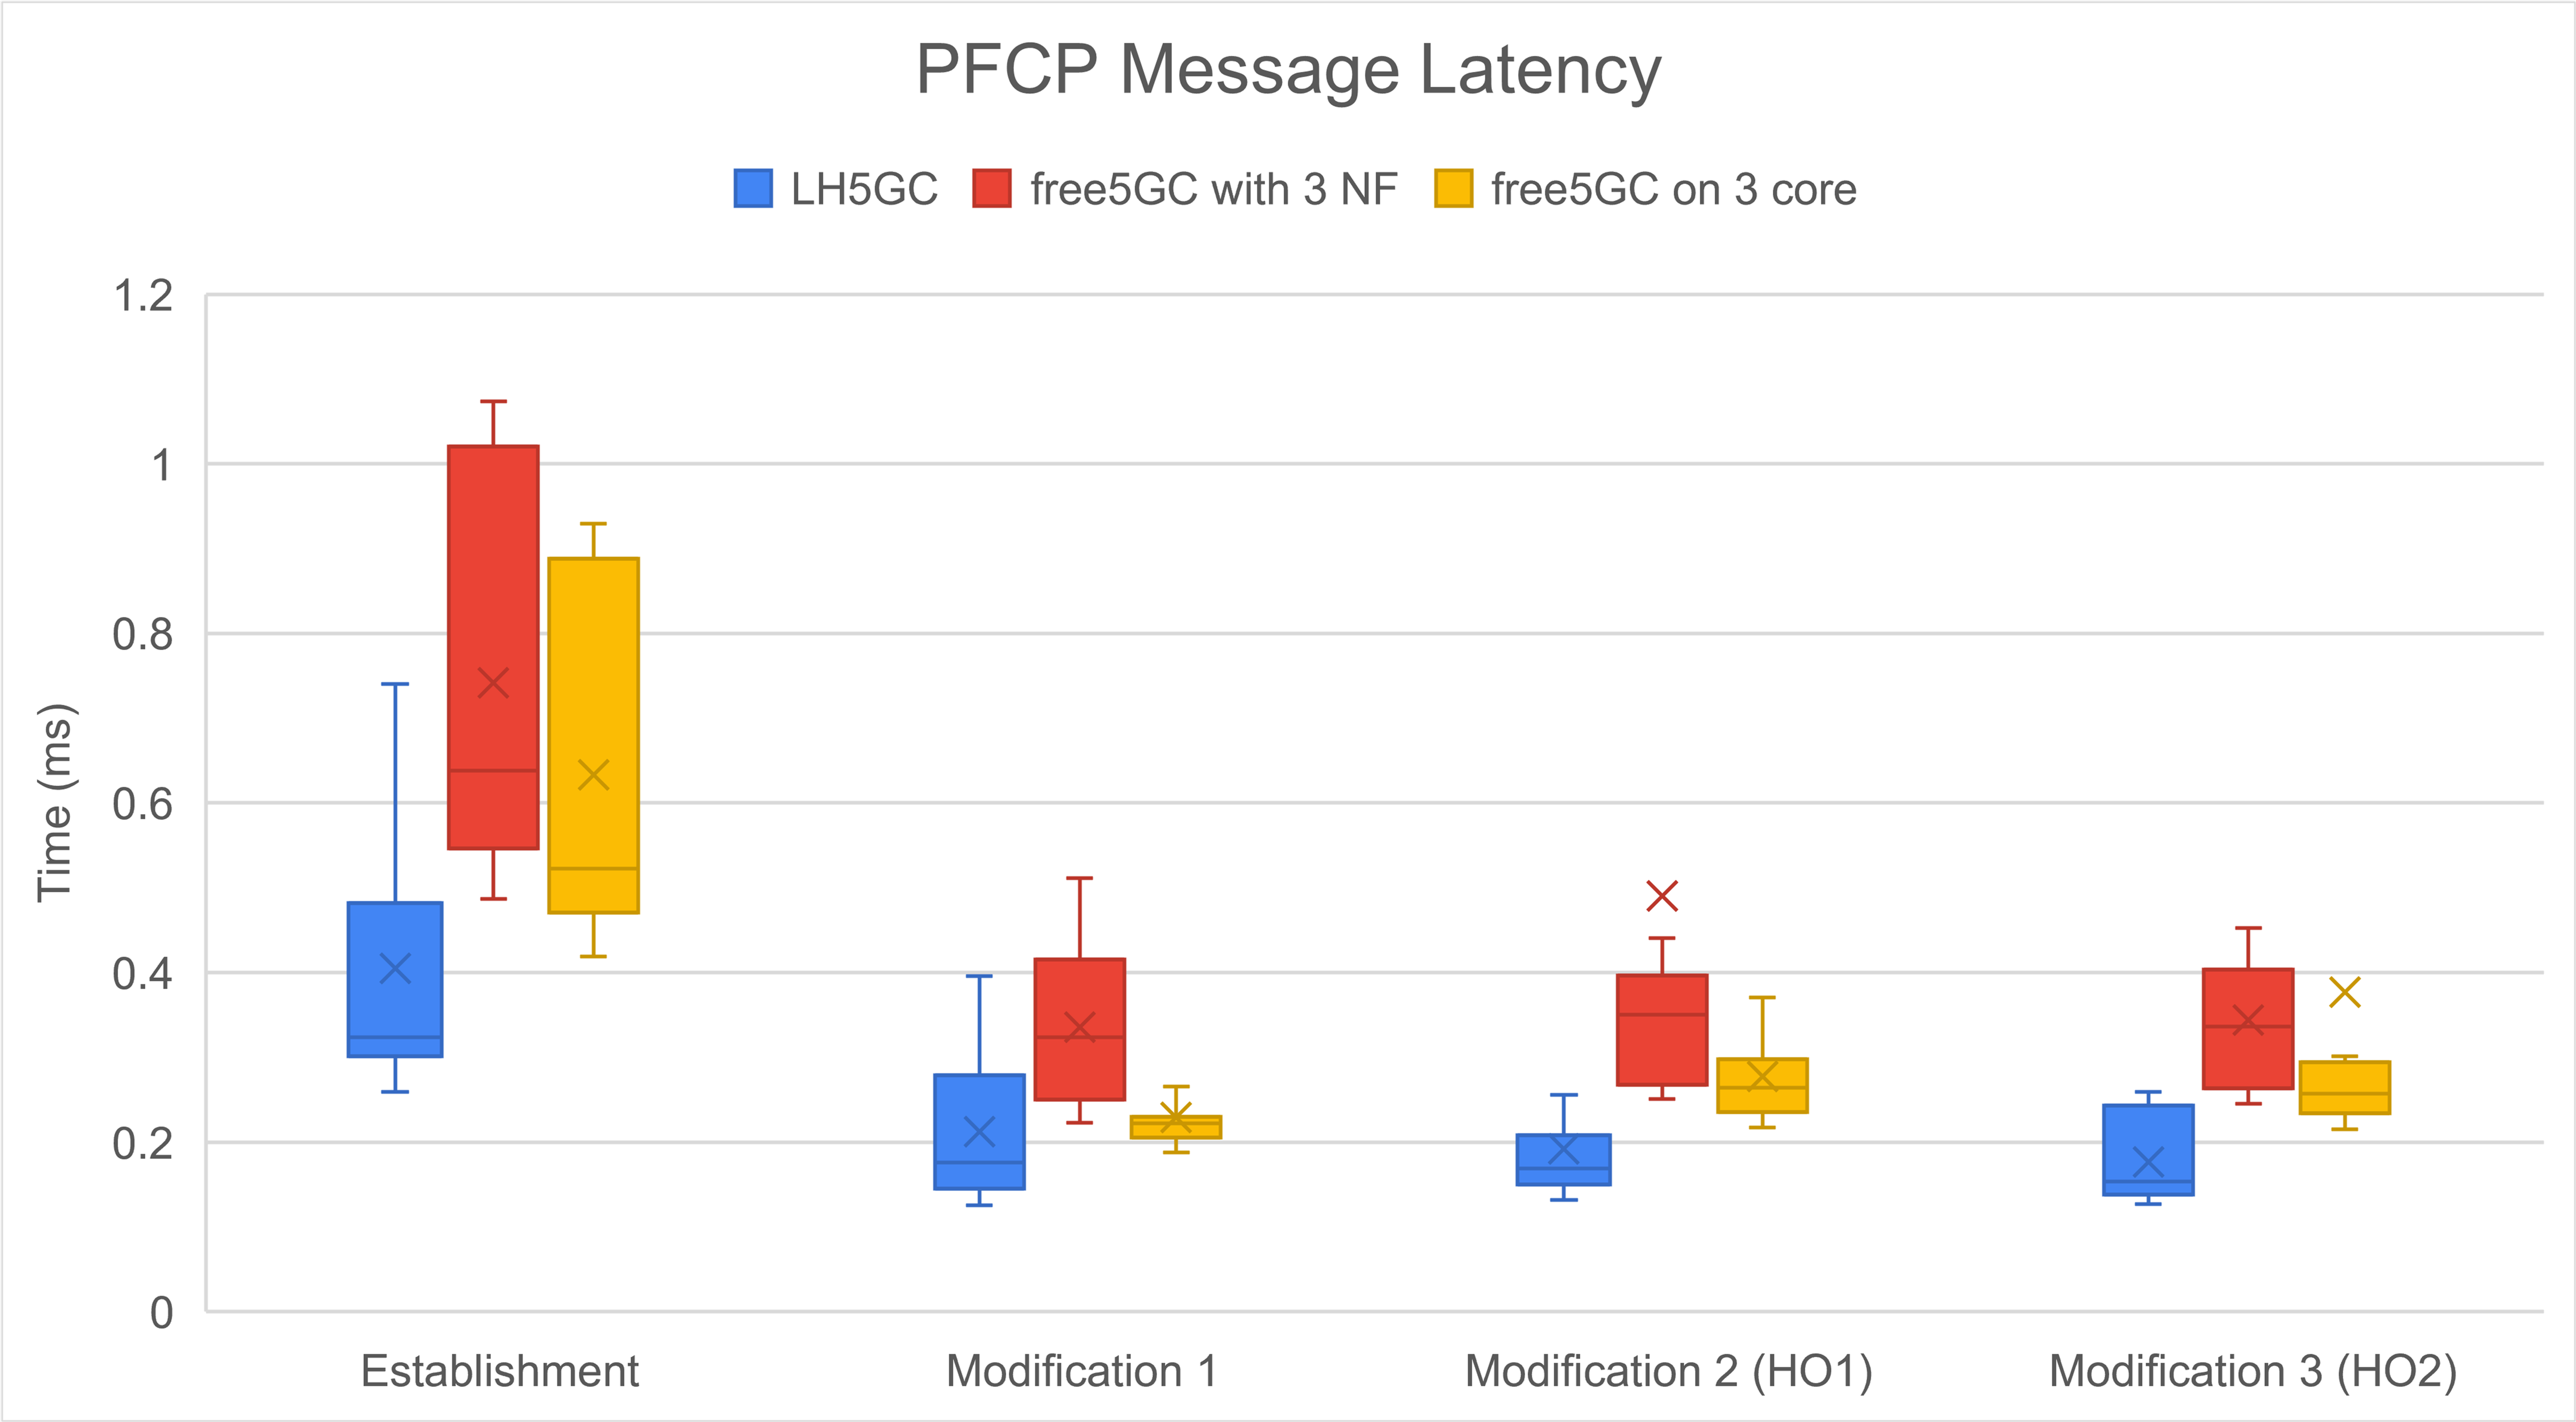
\includegraphics[height=!,width=0.9\linewidth,keepaspectratio=true]{figures/cp_pfcp_comp}
    % [] 放的是顯示在 list of figure 的文字
    % {} 放的是顯示在圖下方的文字
    \caption[PFCP 訊息延遲比較]{{\footnotesize PFCP 訊息延遲比較}}
    \label{fig:cp_pfcp_comp}
\end{figure}

圖\ref{fig:cp_pfcp_comp}的縱軸是時間,取毫秒為單位。可以看出 free5GC 在各信息的平均延遲皆大於 \LHCN 的測試,在 Establishment 訊息上 free5GC 多 \LHCN 1.8 倍的延遲時間、在 Modification 1 上多了 1.5 倍、在 Modification 2 上多了 2.5 被、而在 Modification 3 上多了 1.9 倍的延遲。另外具有 3 個空 NF 的延遲會是最大的,我們認為是因為雖然有 3 個 NF 並沒有功能,但依然會消耗到 CPU 的運算資源。

\subsection{SBI 延遲差異}
\label{subsec:sbi_comp}

在 SBI 延遲測試中,我們選擇測試 SMContextCreate 此單條訊息,此訊息是由 AMF 送至 SMF,用以通知 SMF 開始建立連線的控制訊息。

\begin{figure}[htbp]
    \centering
    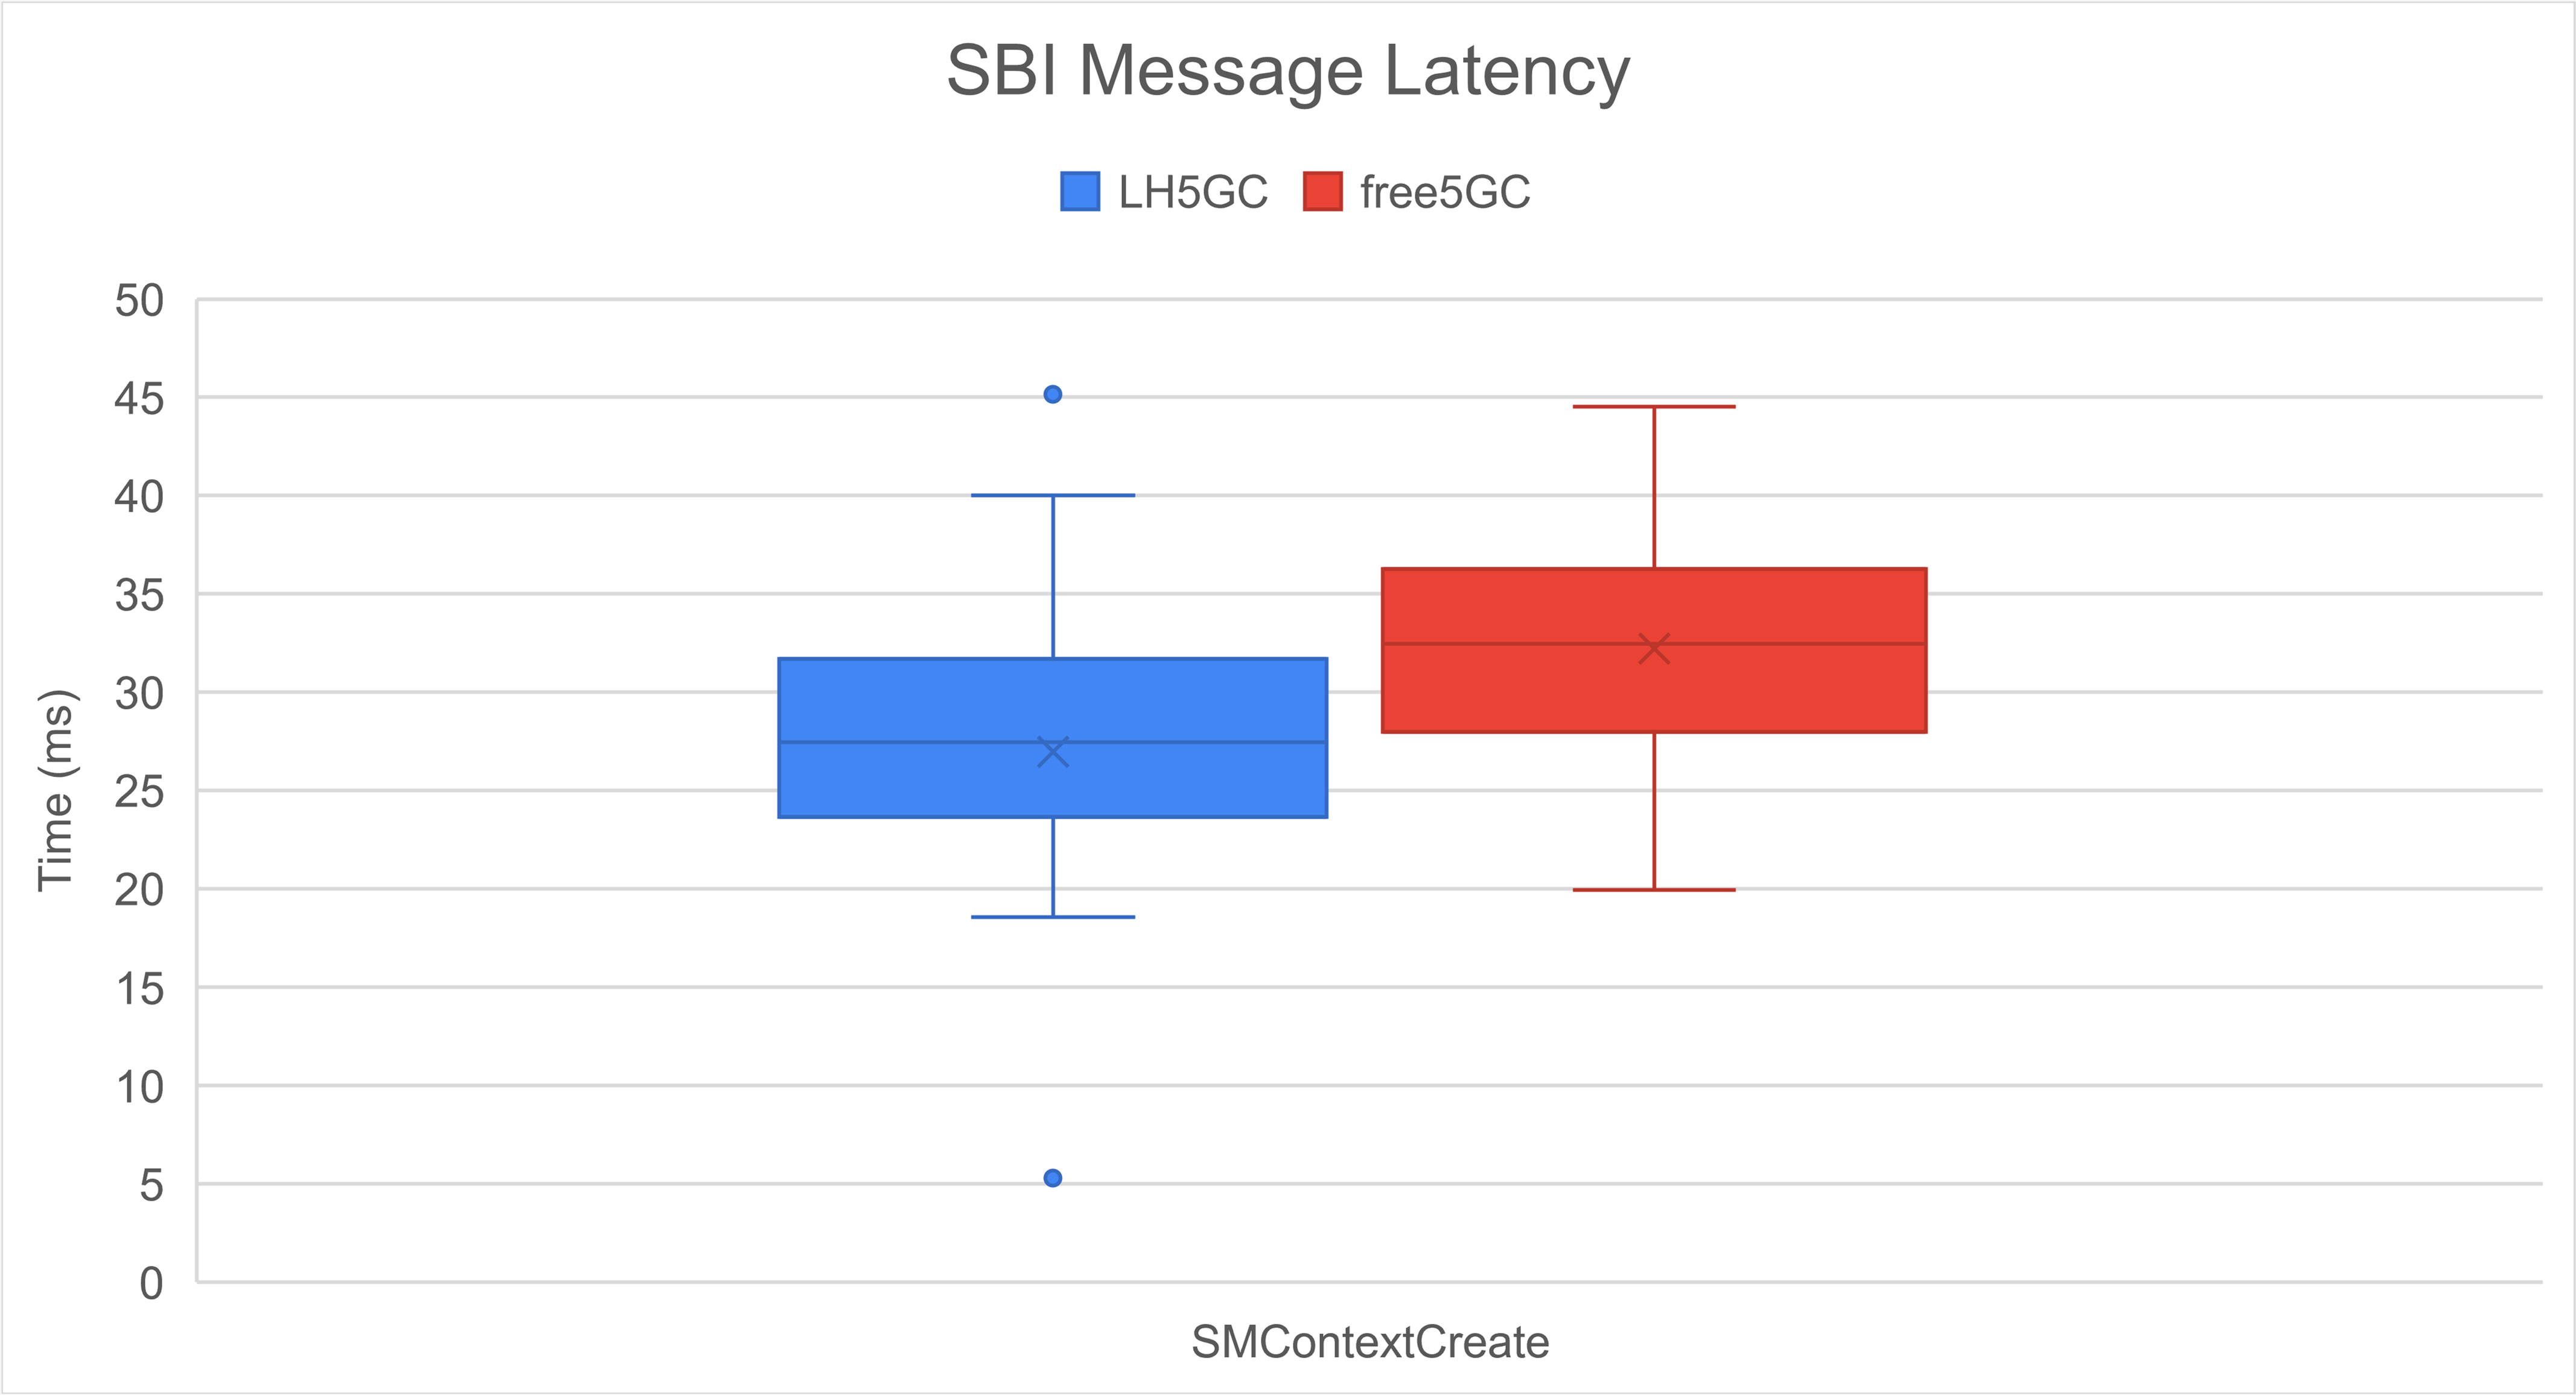
\includegraphics[height=!,width=0.8\linewidth,keepaspectratio=true]{figures/cp_sbi_comp}
    % [] 放的是顯示在 list of figure 的文字
    % {} 放的是顯示在圖下方的文字
    \caption[SBI 訊息延遲比較]{{\footnotesize SBI 訊息延遲比較}}
    \label{fig:cp_sbi_comp}
\end{figure}

\begin{table}[htbp]
    \centering
    \begin{tabular}{|c|c|c|c|}
        \hline
        & \LHCN & free5GC & Processing Delay \\
        \hline
        Average Delay (ms) & 26.95673585 & 32.2257988 & 20.57215 \\
        \hline
        SMF Propagation Delay (ms) & 6.38458545 & 11.6536484 & \\
        \hline
    \end{tabular}
    \caption[SBI 傳播延遲]{{\footnotesize SBI 傳播延遲}}
    \label{tab:cp_sbi_propagation}
\end{table}

圖~\ref{fig:cp_sbi_comp}可看出 \LHCN 透過共享記憶體的方式溝通的效能略優於 free5GC 透過傳統 Kernel Socket 的傳輸,但似乎不太明顯。但若我們嘗試將 NF 的 Processing Delay 扣除 (見表~\ref{tab:cp_sbi_propagation}),則 \LHCN 在 SMContextCreate 訊息的傳播延遲 (propagation delay) 平均會是 6.38 ms,而 free5GC 的平均則是 11.65,可見除了減少溝通延遲,NF 本身的運算速度亦會對總體延遲產生影響。

\subsection{控制流程延遲比較}
\label{subsec:cp_proc_comp}

最後,我們比較控制端三個完整流程的延遲:註冊流程、連線建立流程、以及換手流程。同樣的我們比較的是 \LHCN、free5GC 與在同一系統上開啟 3 個 OpenNetVM 平臺上的無功能 NF、以及 free5GC 只能在三個核心上執行的版本。

\begin{figure}[htb]
    \centering
    \begin{subfigure}[b]{.5\linewidth}
        \centering
        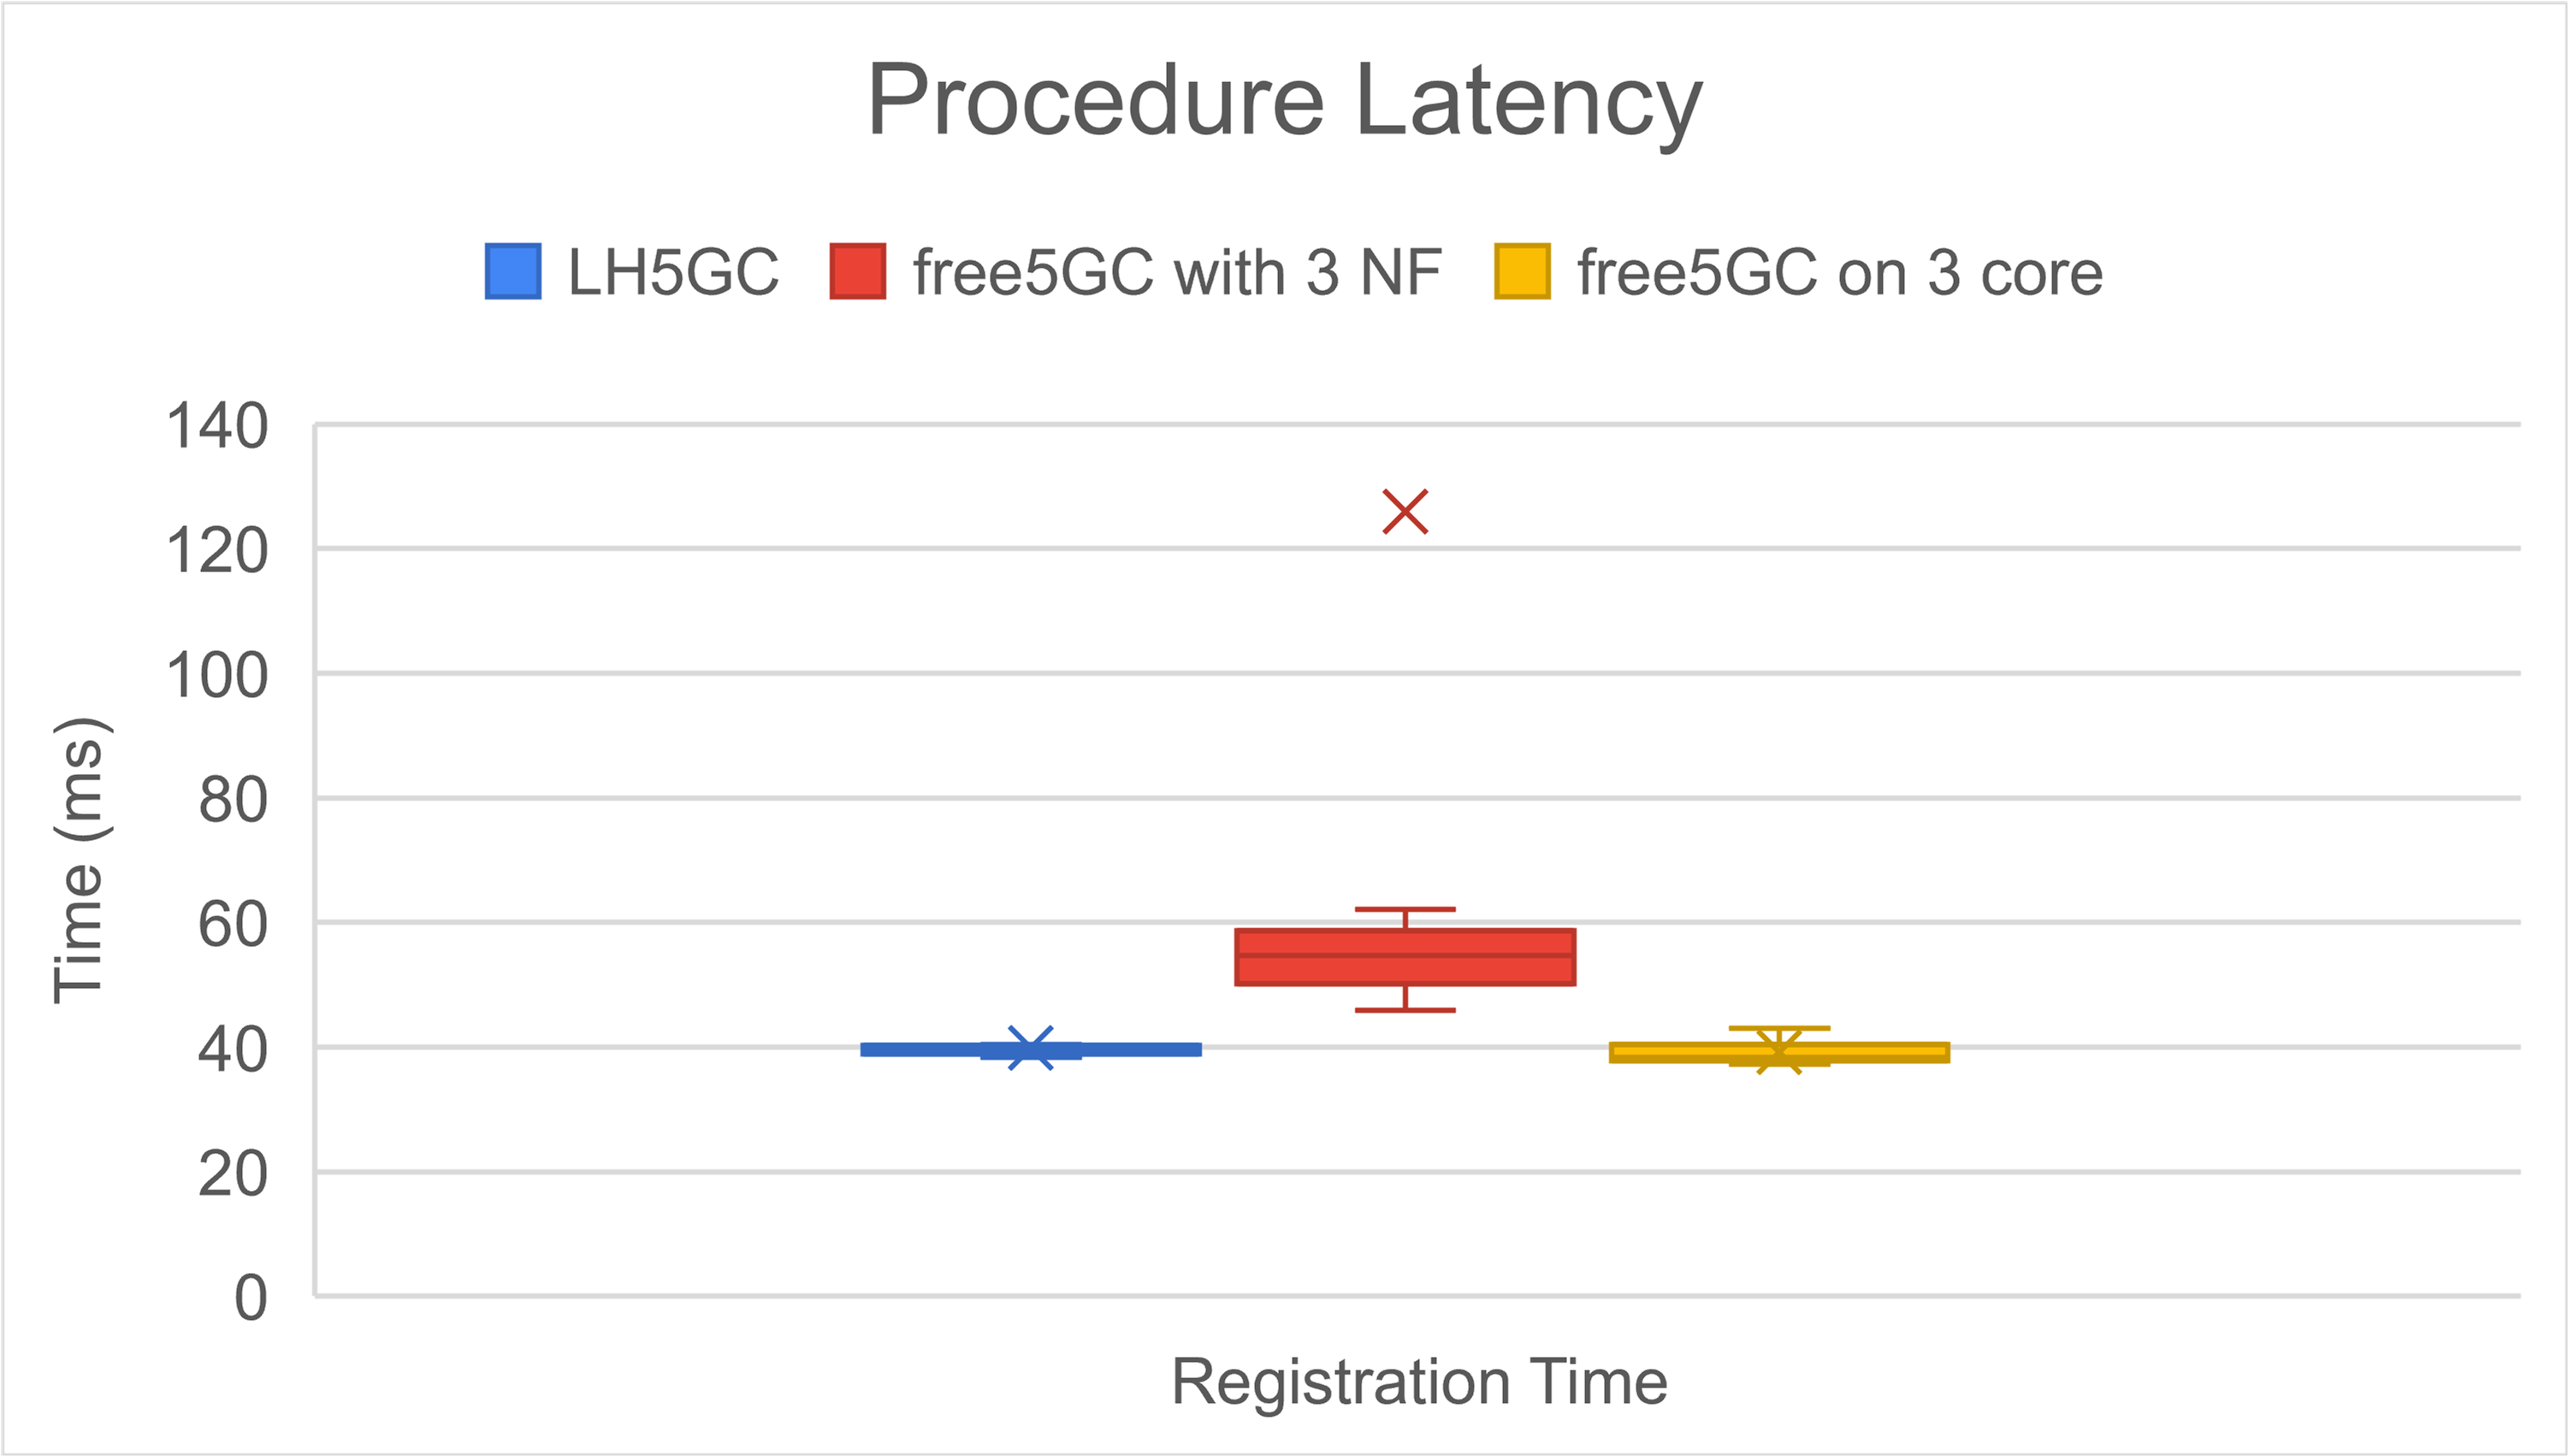
\includegraphics[height=!,width=0.95\linewidth,keepaspectratio=true]{figures/cp_proc_reg}
        \caption[]{{\footnotesize}}
        \label{fig:cp_proc_reg}
    \end{subfigure}%
    \begin{subfigure}[b]{.5\linewidth}
        \centering
        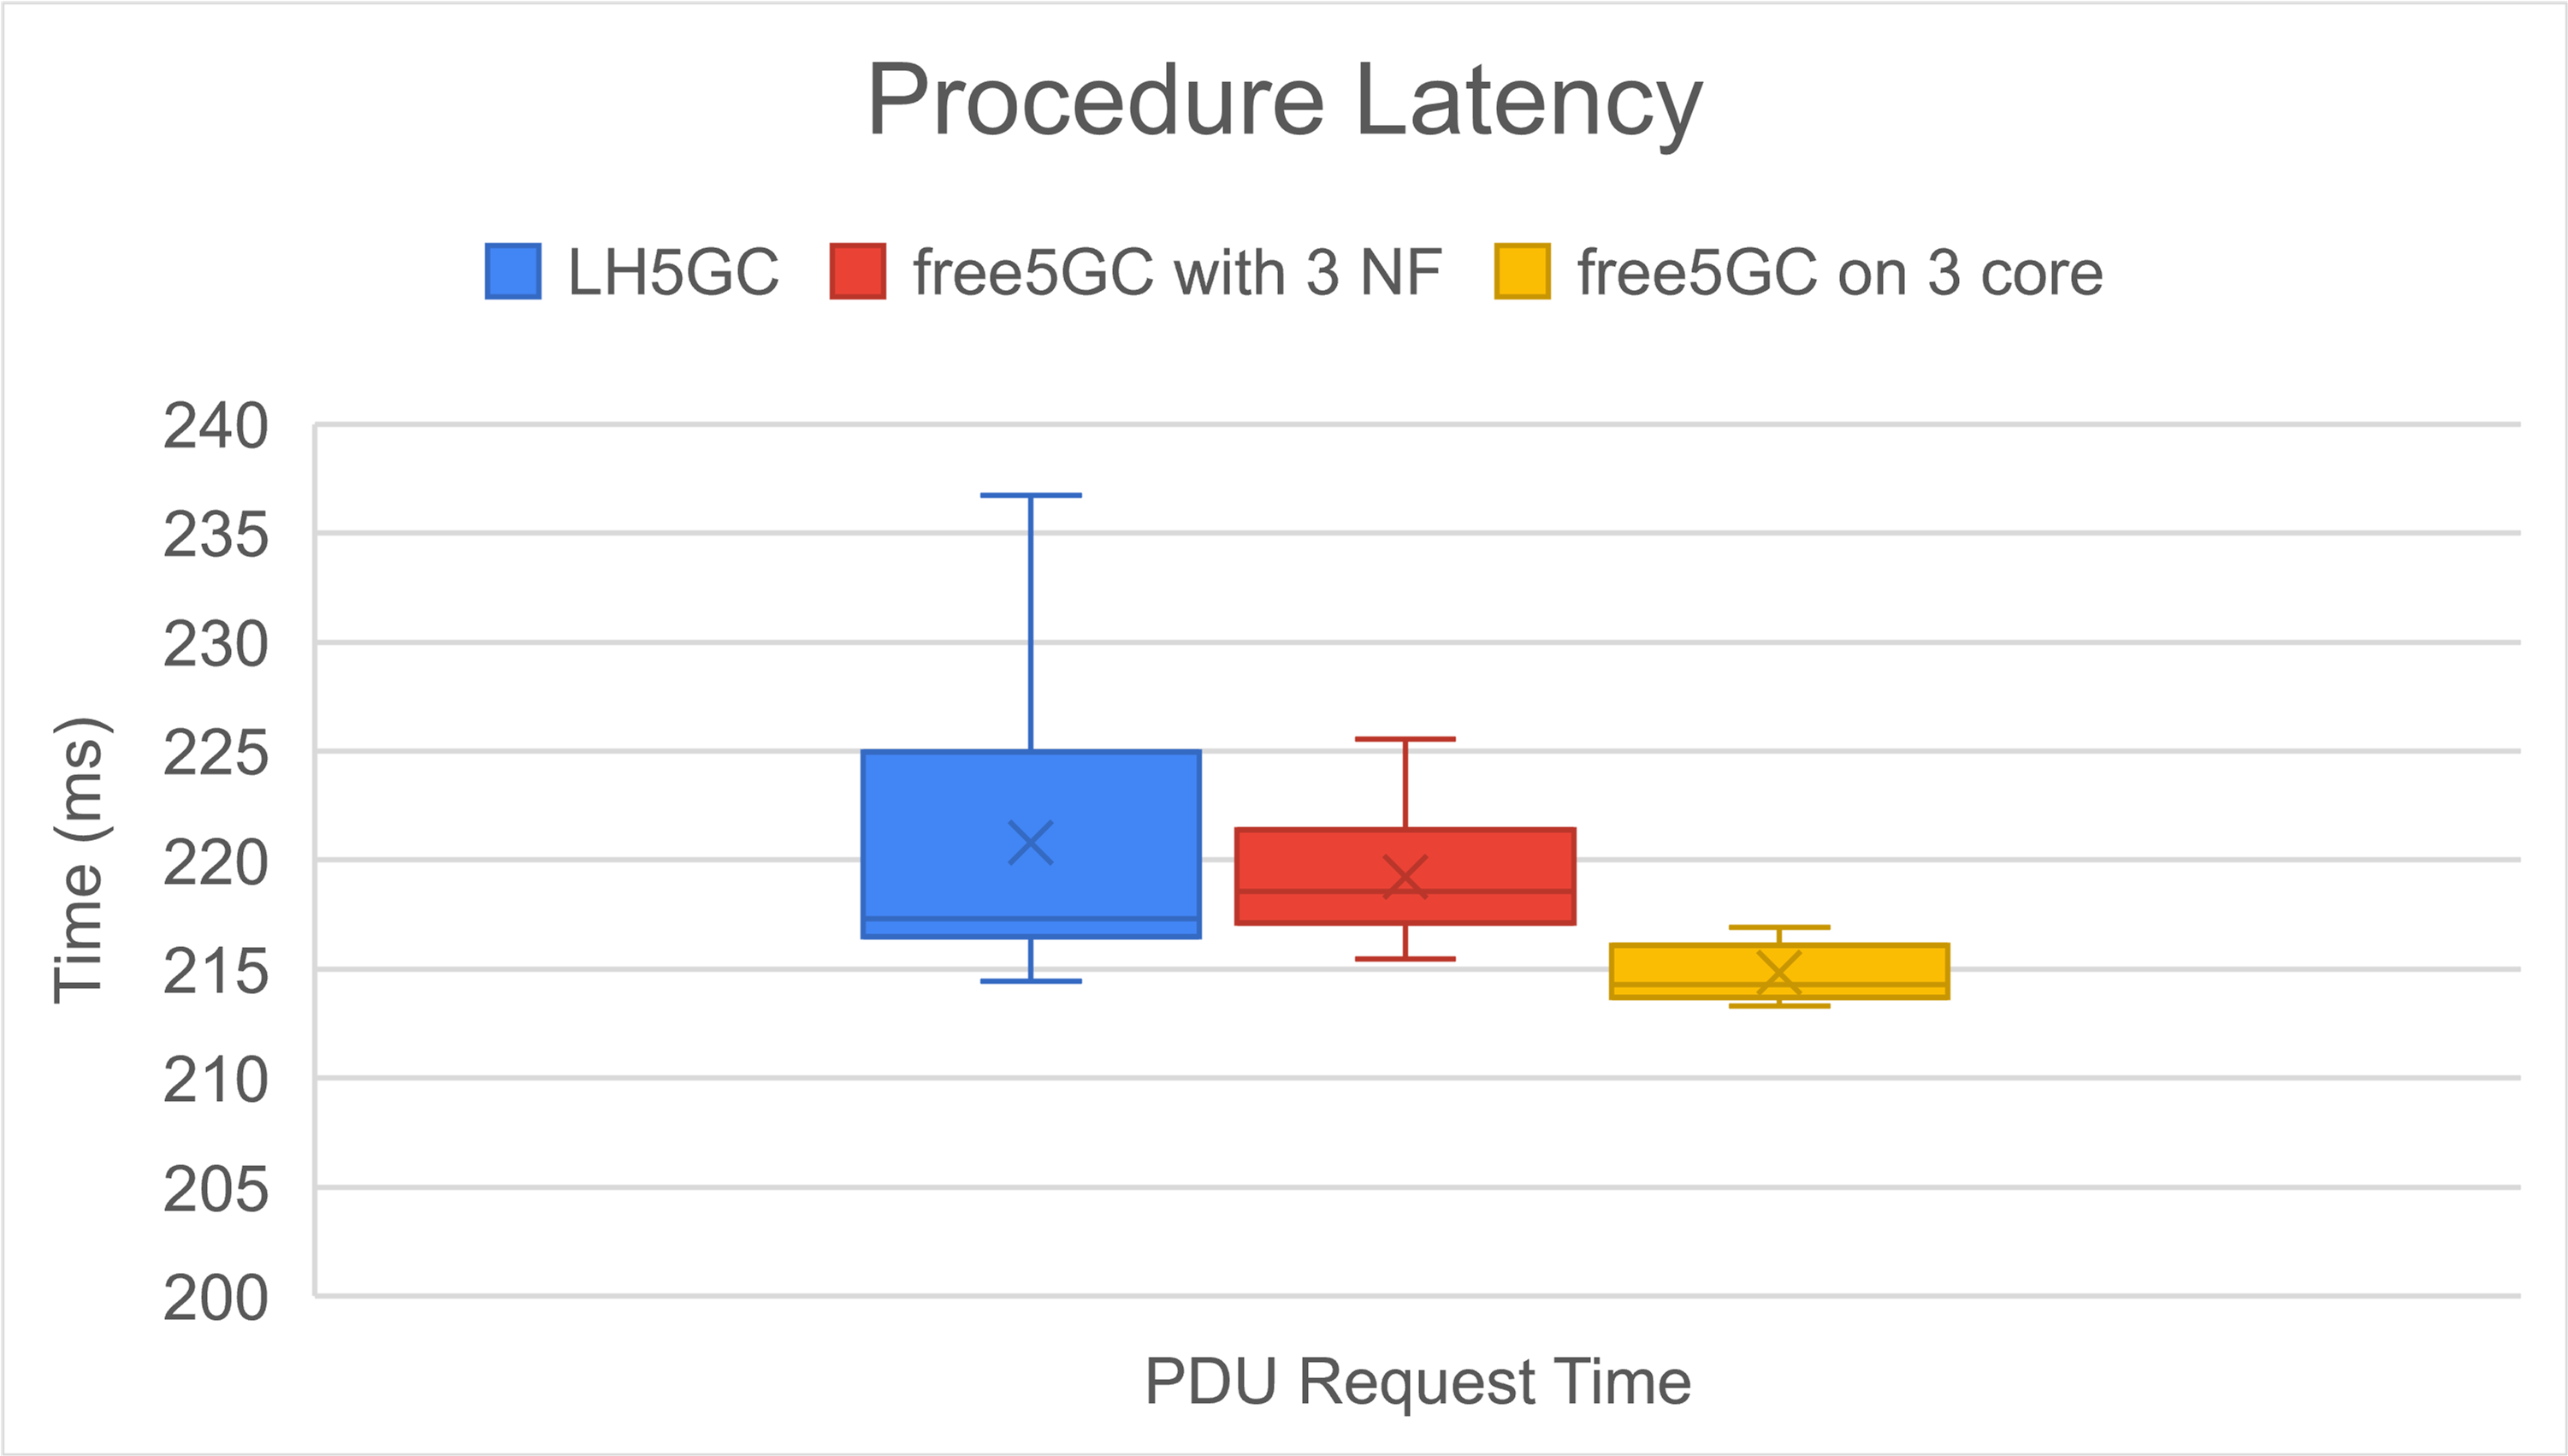
\includegraphics[height=!,width=0.95\linewidth,keepaspectratio=true]{figures/cp_proc_sess}
        \caption[]{{\footnotesize}}
        \label{fig:cp_proc_sess}
    \end{subfigure}
    \begin{subfigure}[b]{.5\linewidth}
        \centering
        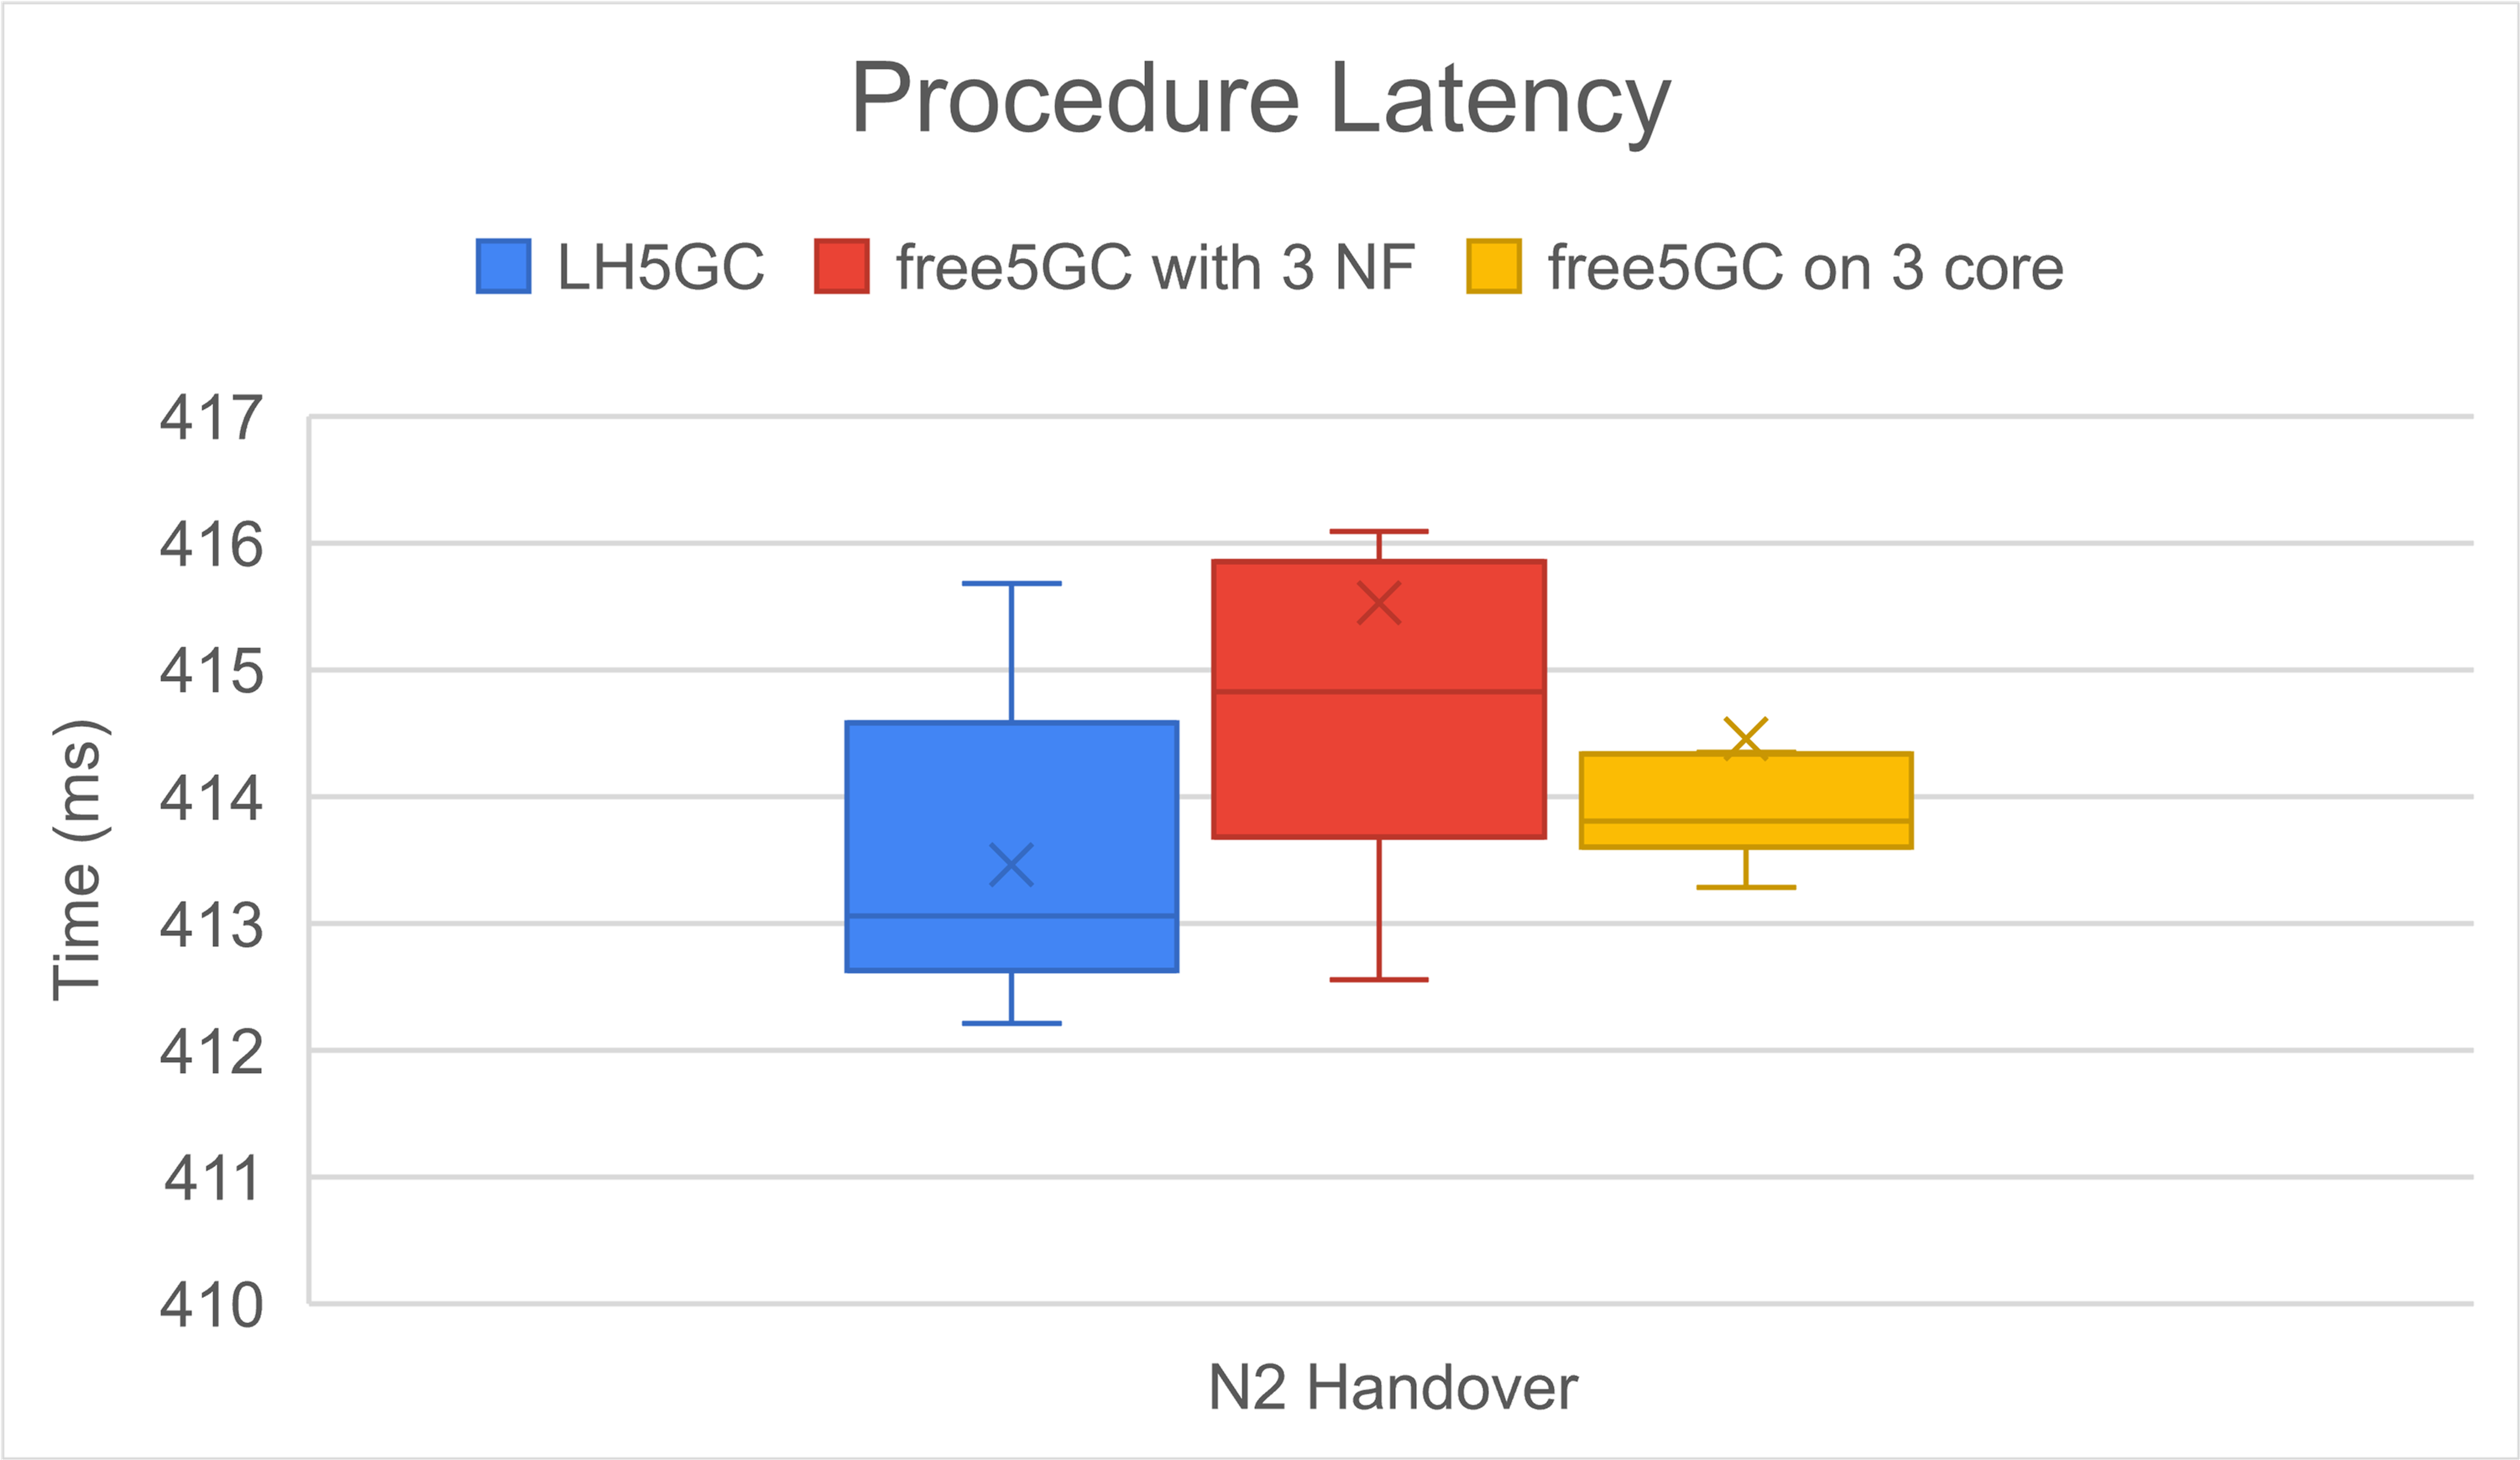
\includegraphics[height=!,width=0.95\linewidth,keepaspectratio=true]{figures/cp_proc_ho}
        \caption[]{{\footnotesize}}
        \label{fig:cp_proc_ho}
    \end{subfigure}%
    % [] 放的是顯示在 list of figure 的文字
    % {} 放的是顯示在圖下方的文字
    \caption[控制流程延遲差異]{{\footnotesize 控制流程延遲差異}}
    \label{fig:cp_proc_comp}
\end{figure}

由圖~\ref{fig:cp_proc_comp}可以看出就整體控制端流程,\LHCN 的平均值會稍微比 free5GC 的兩個測試版本好,然而差別並不大,就其原因可以從觀察 SBI 單一訊息的延遲觀察中發現 (表~\ref{tab:cp_sbi_propagation}),雖然 \LHCN 在訊息傳遞的傳播延遲上好過 free5GC,但就處理延遲 (processing delay) 與傳播延遲 (propagation delay)的比例來看 ($26:6 \approx 4:1$),並沒有獲得很大比例的效益。控制訊號的傳遞延遲需要透過更多訊息累積才能獲得比較好的效益,而目前 \LHCN 僅有在 PFCP 與 SMContextCreate 界面上完成共享記憶體的使用,若可將所有 SBI 移植至共享記憶體上,將會帶來更大的效益。
